%Input preamble
\documentclass[11pt]{article}

% colors
\usepackage[table]{xcolor}
\definecolor{maroon}{RGB}{153,0,18}
\definecolor{lime}{RGB}{190,213,88}
\definecolor{sand}{RGB}{217,202,179}
\definecolor{fire}{RGB}{144,50,61}
\definecolor{brick}{RGB}{94,11,21}
\definecolor{olive}{RGB}{117,109,84}
\definecolor{lavpink}{RGB}{172,123,132}
\definecolor{darkpurp}{RGB}{49,10,49}
\definecolor{salmon}{RGB}{204,90,113}
\definecolor{mauve}{RGB}{94,73,85}
\definecolor{greyblue}{RGB}{125,132,145}
\definecolor{greypurp}{RGB}{68,56,80}
\definecolor{brightpurp}{RGB}{96,20,255}

% packages (please add in alphabetical order)
\usepackage{adjustbox}
\usepackage{amsfonts}
\usepackage{amsmath}
\usepackage{amssymb}
\usepackage{array}
\usepackage{bm}
\usepackage{booktabs}
\usepackage{caption}
\usepackage{epstopdf}
\usepackage{float}
\usepackage[margin=1in]{geometry}
\usepackage{graphicx}
\usepackage[colorlinks=true, linkcolor=brightpurp, citecolor=brightpurp, urlcolor=salmon]{hyperref}
\usepackage{lipsum}
\usepackage{longtable}
\usepackage{mathtools}
\usepackage{multirow}
\usepackage{natbib}
\usepackage{rotating}
\usepackage{setspace}
\usepackage{subcaption}
%\usepackage{threeparttable}
\usepackage{threeparttablex}
\usepackage{xr}
\usepackage[printwatermark]{xwatermark}


\newcolumntype{L}[1]{>{\raggedright\let\newline\\\arraybackslash\hspace{0pt}}m{#1}}
\newcolumntype{C}[1]{>{\centering\let\newline\\\arraybackslash\hspace{0pt}}m{#1}}
\newcolumntype{R}[1]{>{\raggedleft\let\newline\\\arraybackslash\hspace{0pt}}m{#1}}

% commands
\newcommand{\mr}{\multirow}
\newcommand{\mc}{\multicolumn}


\begin{document}

\doublespacing

\noindent Back-of-the-envelope CBA \\
\noindent Analogous to \citet{Kline-Walters_2015_NBER-Evaluating}\\

\noindent This section presents a back-of-the-envelope cost-benefit analysis in a similar spirit to that of \citet{Kline-Walters_2015_NBER-Evaluating} on Head Start, using data from the Head Start Impact Study. For simplicity, we leave CARE out of this exercise. The implementation of \citet{Kline-Walters_2015_NBER-Evaluating} is based on the argument of  \citet{Chetty_Friedman_etal_2010_HowDoesYour} that a standard deviation in a kindergarten IQ score generates an increase of $13.1\%$ in earnings at age 27.\footnote{\citet{Chetty_Friedman_etal_2010_HowDoesYour} do not present a cost-benefit analysis. They (i) present an estimate of the effect that an change in the classroom size has on children's IQ in kindergarten; (ii) link this effect to earnings gains at age 27, by the implied relationship between the gain in IQ and the gain in earnings at age 27 given the change in classroom size.}\\

\noindent We perform two exercises. First, the analogous to \citet{Kline-Walters_2015_NBER-Evaluating}. We calculate the treatment effect of ABC on a kindergarten IQ test---Wechsler Preschool and Primary Scale of Intelligence at Age 5, $\widehat{\Delta}$, and let the (discounted to age 5) life-cycle earnings in 2014 USD dollars be $\$460,793.34$. We take this number straight from \citet{Kline-Walters_2015_NBER-Evaluating}. Based on this, we calculate the total benefits induced by the program as: 

\begin{equation}
B = 460,793.34 \left( \widehat{\Delta} R_{IQ}  N_{\text{Treated}}  -  N_{\text{Control}} \right) , 
\end{equation}

\noindent where $N_{\text{Treated}}$ is the number of subjects in the treatment groups and $N_{\text{Control}}$ is the number of subjects in the control groups. $R_{IQ}$ is the earnings return to a standard deviation increase in a kindergarten IQ test---13.1\% in the case of \citep{Chetty_Friedman_etal_2010_HowDoesYour}. Then, we let the total cost of the program (discounted to age 5) be $\$5,403,133$, as documented in Appendix~\ref{app:programcosts}. We denote this by $C$.\\ 

\noindent For the program to break-even with respect to costs and benefits, a much higher return to the kindergarten IQ test is needed than the one reported in \citep{Chetty_Friedman_etal_2010_HowDoesYour}, $13.1\%$ vs. $ > 40\%$. Figure~\ref{figure:first} plots the relationship between the $B/C$ and various values of $R_{IQ}$.\\ 

\noindent Next, we perform a similar calculation. Instead of letting $R_{IQ}$ vary, we fix it to $13.1\%$ and let the net present value of earnings over the life cycle vary. For the program to break even, this value needs to be beyond a million dollars (Figure~\ref{figuresecond}). \citet{Kline-Walters_2015_NBER-Evaluating} argue that this value is $\$359,064.50$ for disadvantaged populations in the U.S.

\begin{center}
\begin{figure}[H] 
\caption{Benefit-to-cost Ratio and the Earnings Returns to a Kindergarten IQ Test} \label{figure:first}
\centering
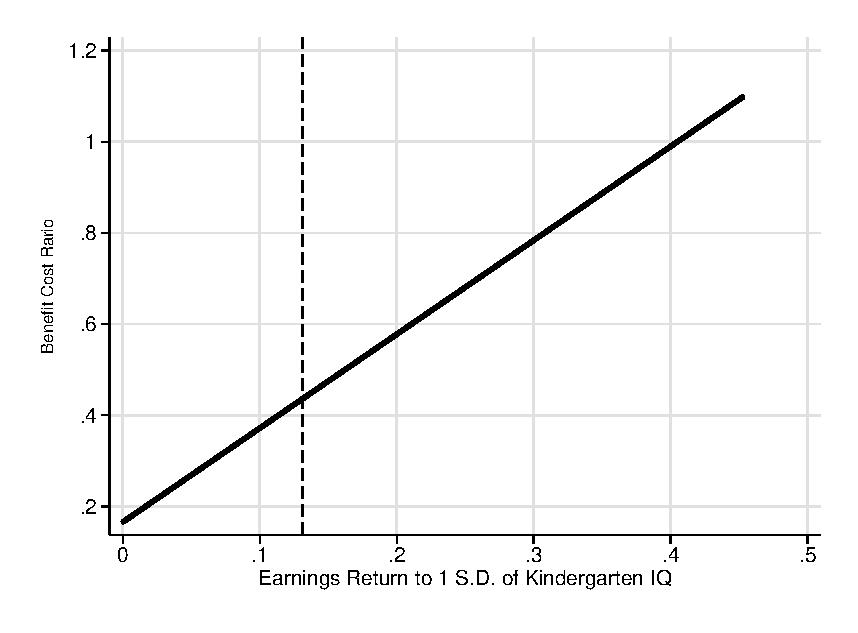
\includegraphics[width=.65\columnwidth]{Output/abc_chettytype_return.eps}
\floatfoot{
\footnotesize
Note: Benefit-to-cost ratio as a function of diverse earnings-returns to a standard deviation of a kindergarten IQ test.
}
\end{figure}
\end{center}

\begin{center}
\begin{figure}[H] 
\caption{Benefit-to-cost Ratio and the Discounted Net Present Value of Earnings}
\label{figuresecond}
\centering
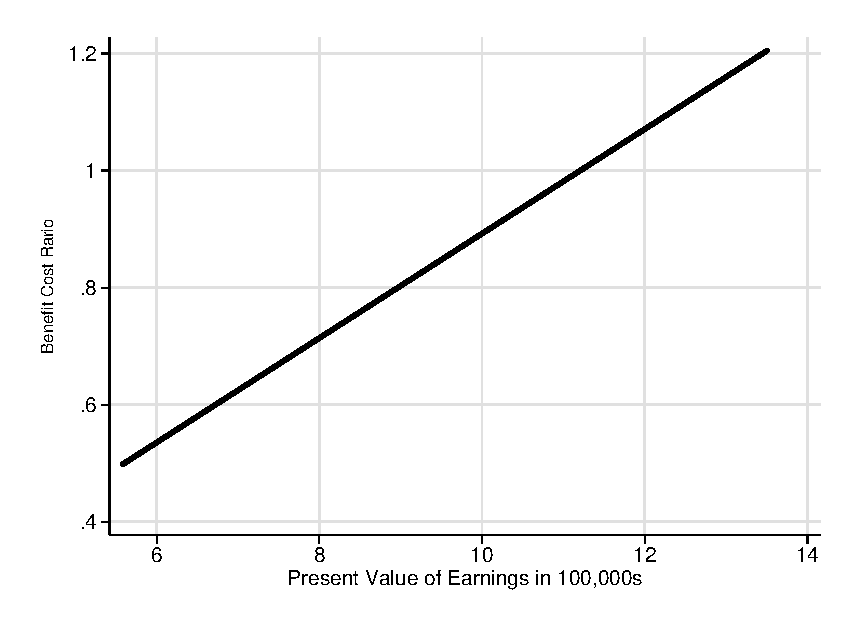
\includegraphics[width=.65\columnwidth]{Output/abc_chettytype_pv.eps}
\floatfoot{
\footnotesize
Note: Benefit-to-cost ratio as a function of diverse net present value of earnings.
}
\end{figure}
\end{center}

%References
\singlespace
\bibliographystyle{chicago}
\bibliography{heckman}
\end{document}